\documentclass[10pt]{article}
\usepackage[utf8]{inputenc}

%Márgenes y tipo de hoja
\usepackage{geometry}
\geometry{letterpaper,portrait,
rmargin=20mm, 
lmargin=20mm,
bmargin=20mm,
tmargin=0mm,
headheight=0mm}
\renewcommand{\headrulewidth}{0pt}
\usepackage{graphicx}
\usepackage{wrapfig}
\usepackage{float}

% Logos
\usepackage{fontawesome}

%Header
\usepackage{xcolor}
\usepackage{fancyhdr}
\pagestyle{fancy}
\fancyhf{}

% Tipo de letra y color
\usepackage{PTSansNarrow} 
\renewcommand*\familydefault{\sfdefault}
\usepackage[T1]{fontenc}
\usepackage{xcolor}
\usepackage{anyfontsize}

% Indentacion de parrafos completos
\usepackage{changepage}

% Paquete para columnas multiples
\usepackage{multicol}
\setlength{\columnsep}{10pt}
 \usepackage{vwcol} 

% Indentacion y otras longitudes
\setlength{\parindent}{0pt}
\setlength{\parskip}{10pt}
\renewcommand{\baselinestretch}{1}

% Figura
\usepackage{tikz}

\begin{document}
\begin{tikzpicture}[remember picture,overlay]
   \node[anchor=north,inner sep=0pt] at (current page.north)
   \draw[blue, very thick] (-5,-3.1) rectangle (50,5);
   \filldraw[fill=blue!50!black, draw=blue!50!black](-5,-3.1) rectangle (50,5);
\end{tikzpicture}
\begin{tikzpicture}[remember picture,overlay]
   \node[anchor=north east,inner sep=0pt] at (current page.north east)
              {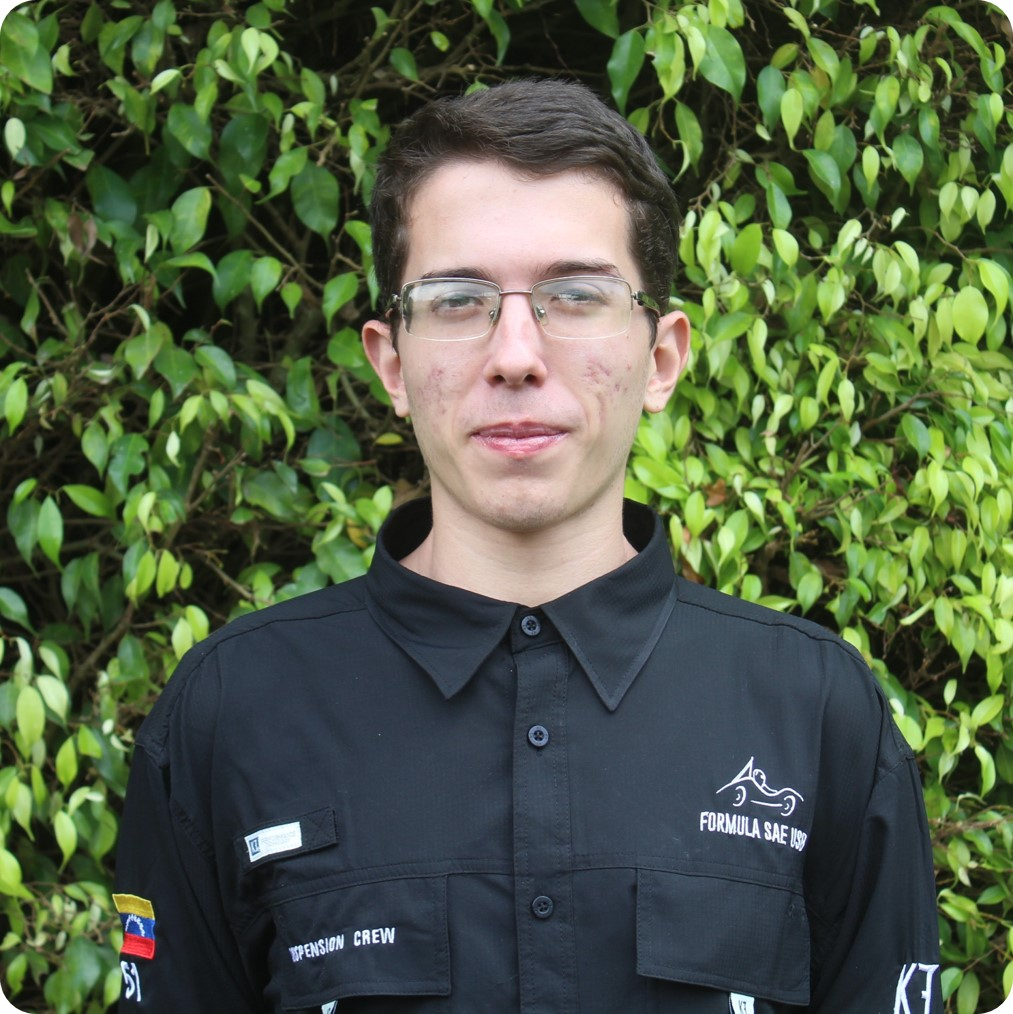
\includegraphics[scale=0.2]{foto/foto_perfil.JPG}};
\end{tikzpicture}

\begin{center}
\color{white}
{\fontsize{40}{60}\selectfont Jesús \textbf{Pereira}}
\vspace{2pt}\\
\vspace{2pt}
\faMapMarker\hspace{3pt}Caracas\hspace{25pt}|\hspace{25pt} Venezuela\hspace{25pt}|    \hspace{25pt}\faMobile\hspace{2pt} +58 424 1234715\\
jesusepereira@gmail.com\hspace{25pt}|\hspace{25pt}\faLinkedinSquare\hspace{3pt}/in/jeppires/\hspace{25pt}|\hspace{25pt} \faGithubSquare\hspace{3pt}/jesusepp    
\end{center}
 \vspace{20pt}
\begin{multicols}{2}

\begin{LARGE}
\color{blue!50!black}
Habilidades\par
\end{LARGE}
\begin{multicols}{2}
\textbf{Lenguajes y\\
Frameworks:}\par
\textbf{Herramientas de diseño:}\par
\hfill\par
\begin{flushleft}
LaTeX, MATLAB, Python, HTML, CSS.\par
SolidWorks, ANSYS Mechanical, ANSYS Fluent.\par
\end{flushleft}
\end{multicols}
\hfill\par
\hfill\par
\columnbreak
\begin{LARGE}
\color{blue!50!black}
Informacion Personal\par
\end{LARGE}
Actual estudiante de 10mo trimestre en Ingenieria Mecánica, miembro del equipo de fórmula SAE de la univeridad Simón Bolívar, apasionado del aprendizaje y capaz de resolver problemas que requieran trabajo en equipo y cooperación.\par
\begin{LARGE}
\color{blue!50!black}
Idiomas\par
\end{LARGE}
\begin{multicols}{3}
\textbf{Español}\\
\textbf{Inglés}\\
\textbf{Alemán}\\
Nativo\\
Avanzado\\
Básico\\
\hfill\par
\hfill\par
\end{multicols}
\end{multicols}

\begin{multicols}{2}
\begin{LARGE}
\color{blue!50!black}
Cursos\par
\end{LARGE}
\begin{multicols}{2}
\hspace{5pt}Oct/2019\\
\hfill\par
\hspace{5pt}Abr/2020\\
\par
Certificación en SolidWorks, examen del CSWA.\par
Certificación en el EF SET con 80/100.\\
\end{multicols}
\columnbreak
\begin{LARGE}
\color{blue!50!black}
Educación\par
\end{LARGE}
\begin{multicols}{2}
\hspace{5pt}Abr/2016 - Present\\
\hfill\\
\hfill\\
\hfill\par
\hfill\par
\textbf{Ingeniería Mecánica}\\
Universidad Simón Bolívar\\
160 unidades-crédito\\
Índice Académico: 4.9/5
\end{multicols}
\end{multicols}
\begin{LARGE}
\color{blue!50!black}
Experiencia Laboral\par
\end{LARGE}
\begin{vwcol}[widths={0.22,0.78},
 sep=.8cm,rule=0pt,indent=0em,lines=6] 
\hspace{5pt}Jul/2018 - Jun/2019\par
\hfill\\
\hfill\\
\hfill\\
\hfill\\
\hfill\\
\textbf{Miembro de la división de Suspensión}\hfill \textit{FSAE USB}\\
Esta división es la encargada del diseño, construcción y seteo del sistema de suspensión de un prototipo Formula Student construido por FSAE USB. Junto con los demás miembros de la división, se trabajó en equipo para lograr un sistema funcional, con ayuda de softwares de diseño como SolidWorks, y herramientas de taller como tornos, fresadoras, y equipos de mecánica básicos (llaves, tornillería, entre otros).\par
\end{vwcol}
\begin{vwcol}[widths={0.22,0.78},
 sep=.8cm, rule=0pt,indent=0em,lines=8] 
\hspace{5pt}Jul/2019 - Presente\par
\hfill\\
\hfill\\
\hfill\\
\hfill\\
\hfill\\
\hfill\\
\hfill\\
\textbf{Director de la división de Chasis}\hfill \textit{FSAE USB}\\
Como director de Chasis, se heredan las responsabilidades de diseñar, construir y verificar los diversos sistemas encargados para esta división, entre ellos el frame y sus conexiones con los diversos sistemas del carro y los elementos de seguridad requeridos por la competencia (atenuador de impacto, material absorbente de impactos, entre otros). Es de suma importancia para este cargo tener una buena comunicación con los demás jefes de división, ya que Chasis se encarga de unirlos y evitar que puedan existir problemas entre ellas.\par
\end{vwcol}
\begin{LARGE}
\color{blue!50!black}
Proyectos\par
\end{LARGE}
\begin{vwcol}[widths={0.22,0.78},
 sep=.8cm, rule=0pt,indent=0em,lines=4] 
\hspace{5pt}Abr/2020\par
\hfill\\
\hfill\\
\hfill\\
\textbf{Buscaminas en Python}\hfill\textit{https://github.com/jesusepp/minesweeper\\} 
A través del lenguaje de programación Python, y con la finalidad de probar las capacidad adquiridas para desempeñarse con este lenguaje, se realizó una versión para el terminal de este popular juego. Los resultados fueron aceptables.\par
\end{vwcol}
\end{document}
